\chapter{Cosy SLAM}
\label{chp:cosyslam}
\minitoc
\bigskip


In this chapter, we present an object-level visual-inertial SLAM system based on the deep-learning-based pose estimation CosyPose \cite{labbe2020cosypose}.
We present experimental results from our paper \cite{debeunne2021cosyslam}.

\section{Introduction}
Navigation of legged robots using onboard exteroceptive sensors has gained a lot of traction in recent years due to their progressive deployment for 
industrial applications \cite{bellicoso2018advances}. 
For repeated travels, the map-less teach and repeat methods \cite{furgale2010visual, mattamala2021learning} avoid the need for a metric and globally coherent localization 
by benefiting from the knowledge of a human operator. This works very well for applications in which such supervision is available, and a global map is not. 
% However, many times, in industrial environments, a map is obtainable as a CAD model or 3D scans, in which important assets can be labeled.
Building a metric and semantic map of the environment may be useful to automatize navigation and exploration in larger environments. Besides,
standard objects whose CAD model is known (such as gauges, valves, stairs, etc.) may often appear.

Many representations of the environment are possible depending on the needs of the system. In \cite{fallon2014drift} a prior map defined as a LIDAR point cloud is 
used in a Gaussian particle filter to localize a humanoid robot and perform online foot planning. Fankhauser \cite{fankhauser2014robot} takes as an input 
an external odometry source to produce efficient robot-centric elevation maps while \cite{kim2020vision} builds a global height map to navigate through cluttered 
environments. Other approaches \cite{wisth2021vilens} rely on a tight fusion between proprioceptive and exteroceptive sensors to make the odometry more robust. 
A full overview of these systems can be found in our literature review (\secRef{sec:environment_awareness}).

\begin{figure}[h]
  \centering
  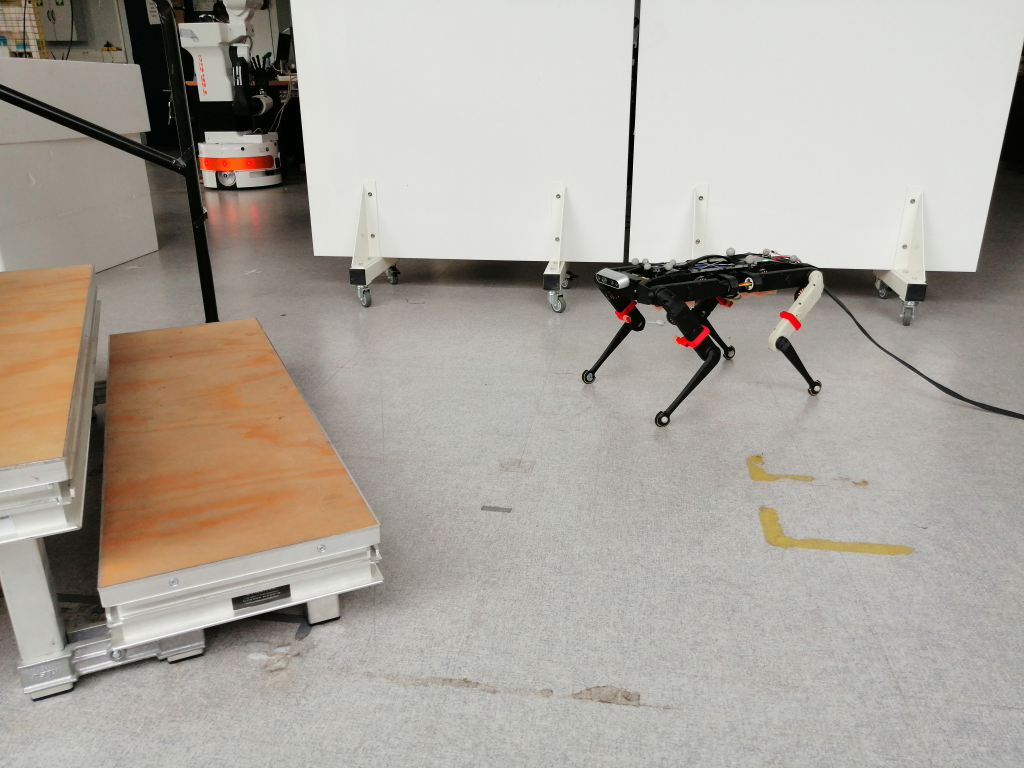
\includegraphics[width=0.80\textwidth]{figures/cosyslam/solo_closer_small.png}
  \caption{Experimental setup: a RealSense D435i is mounted on the Solo robot that localizes itself \wrt stairs. A motion capture system provides ground 
            truth of the robot pose.}
  \label{fig:solo_and_stairs}
\end{figure}

These approaches build metric maps that do not usually leverage the presence of known assets in the scene, although a few examples in the computer vision literature 
exist. In \cite{SalasMoreno2013SLAMSL}, the authors develop one of the first object-level SLAM algorithms from a depth sensor. Using a voting process based on point cloud descriptors, 
a simultaneous recognition and pose estimation of known objects was performed and included as factors in a graph optimization estimator. 
The method benefited from an active search of the objects in the scene, the detection being done in the SLAM loop.
Aside from the robot trajectory and poses of objects, \cite{sucar2020nodeslam} also proposes to optimize the object shapes using a differentiable 
rendering engine. In such approaches, objects need to be detected, classified, and their relative pose \wrt the camera has to be integrated into the estimator. 
On the other end, a work like \cite{pillai2015monocular} uses a semi-dense mono camera SLAM algorithm to produce a scale-ambiguous feature map. 
Then, a descriptor-based multi-view object proposal is performed as a post-processing step. 



% Huge progress to the field of object detection was brought about by the advent of CNN frameworks such as \cite{he2018mask}. As a result, it seems that the domain of 
% object scene reconstruction is now dominated by methods relying only on RGB cameras, for both object detection and pose retrieval. A major example is the framework CosyPose 
% \cite{labbe2020cosypose}. This approach mixes a new state-of-the-art single-view pose estimation algorithm with a multi-view algorithm using RANSAC and Bundle Adjustment. 
% It achieved first in most of the 2020 BOP challenge categories \cite{hodavn2020bop}. This system obtains precision in the order of centimeters on real objects whose 3D 
% model is known. 
% Its performances make it a good candidate as a direct 6D pose sensor to perform the multi-sensor fusion. In the context of legged robots, this is very useful to localize the 
% robot \wrt objects it needs to interact with, such as objects to manipulate or stairs to climb. 
% %However, due to a current lack of generalization capability, the trained models cannot be directly used for objects that are not part of its training.
% While these models are not yet able to be generalized to classes of objects, rapid progress is expected in this direction. Their performances are already very interesting 
% to help with the locomotion in known scenes.

%Another thing that is not handled by CosyPose was the assessment of the uncertainty of measurements from the different objects in the scene, which depends on a variety 
% of parameters such as object occlusion and distance. 
% When considering merging a tracker such as CosyPose with other sensor modalities, an important aspect is to predict covariance representing the level of confidence in 
% the tracker estimate.
% Such data uncertainty awareness has been shown to be crucial to the robustness of SLAM systems involving neural networks subsystems such as \cite{yang2020d3vo}, 
% while \cite{SalasMoreno2013SLAMSL} claimed to compute a covariance matrix approximated as the inverse of the Iterative Closest Point output. The methods targeted for 
% deep learning applications are harder to implement, especially if the goal is to use an off-the-shelf pose estimation neural network, as is the case for this paper. 
% For instance, Bayesian Neural Networks \cite{jospin2020hands} need to be trained explicitly for uncertainty prediction while Monte Carlo (MC) Dropout \cite{gal2016dropout} 
% requires multiple forward passes at run-time.


As described in \secRef{sec:object_pose_est_algos}, deep-learning-based object detection systems have now reached an accuracy that makes them candidates for mobile robotics applications.
Applications range from robot manipulation, like sorting known objects, or localization \wrt known assets. For this last application, however,
the direct output of CosyPose is not sufficient for two reasons. First, many objects have strong symmetries, which makes CosyPose orientation estimation jumps from one to the other
depending on the frames. This output has, therefore, to be filtered using prior knowledge about the world or the robot's movements. Second, the robot needs to keep
a memory of objects it has seen when they go out of its field of view.

We present in this chapter a practical implementation of the proposed MAP formulation fusing inertial measurements and object-level visual features estimated
by CosyPose. The stake is to demonstrate that a centroidal filter is able to merge information typically used for balance control (IMU related)
with features typically needed by a high-level planner, \eg the stair steps locations extracted by the object pose estimator.
Beyond the practical validation for legged robots, this also demonstrates that the single view CosyPose can be extended to a sequential
tracker able to benefit from complementary measurements such as an IMU.

To integrate CosyPose measurements with other sensors, we used the noise model based on empirical data, presented in \secRef{sec:cosypose_covariance}. 
We also detail here the pragmatic implementation of heuristics to circumvent outliers in the network output. 
Experimental validations were conducted with a visual-inertial system, first handheld then mounted on a quadruped robot. Finally, we fine-tuned the pre-trained models 
to perform stairs localization, as explained in \secRef{sec:retraining_with_stairs}. 




\section{Implementation of the Visual Inertial filter}

\subsection{Factor Graph formulation}
This section will be very short so as not to repeat ourselves: the problem has the same structure as the \apriltag-IMU VI system presented in \chpRef{chp:absolute_vi}, 
thus it as the same factor graph \figRef{fig:VI_factor_graph}. The \apriltag\ pose measurement model is replaced by the CosyPose measurement model, presented in \secRef{sec:learning_based_object_pose_est}.


\subsection{Data association and Outlier rejection}
A key part of our SLAM system is the association of landmarks with the rejection of erroneous pose estimates. First of all, each object is associated with a 
label $\alpha$ so that a detection can only match a landmark with the same label. Then, the position of the robot is propagated by integrating the IMU measurements 
with the current biases estimates. Thus, each detected object pose can be transformed in the world frame using the propagated robot state. We check if this pose is 
similar to the one of a landmark with the same label with a threshold on the distance between the poses in $SE(3)$. 
If a detection does not match any landmark then a new landmark is created.

CosyPose can return poses of objects that are not included in the scene because of false detections, of Mask-RCNN, or wrong pose estimations (most often due to object symmetries). 
To handle these outlier detections, each landmark is associated with a score $c$ that corresponds to its repeatability over time: 

\begin{equation}
    c = \frac{n_f}{\Delta t}
\end{equation}

$\Delta t$ is the time since the landmark initialization and $n_f$ is the number of factors associated with it.
The lowest scores are filtered with a threshold determined empirically and the associated landmarks are removed from the map.




\section{Experimental validation}

We have produced datasets in the robotic experimental arena at LAAS-CNRS in Toulouse. This is a 3D environment about $10 m \times 5m$ made of flat floors, 
stairs and beams. The robot environment was augmented with objects of the datasets that were used to train CosyPose. Each dataset is composed of three data sources:

\begin{itemize}
    \item A sequence of RGB images (30 Hz)
    \item A sequence of IMU measurements (200 Hz)
    \item A sequence of motion capture (MoCap) measurements (200 Hz), used as ground truth 
\end{itemize}

We recorded two types of datasets: one for the uncertainty models and one for SLAM experiments. For the uncertainty models, reflective MoCap markers 
were attached to the object to obtain the ground truth of their pose. For the SLAM, only the camera was tracked. We used the monocular RGB camera and the Bosh BMI085 
IMU of an Intel RealSense L515 Camera for handheld trajectories. The Intel RealSense d435i was used with the same modalities 
for the experiments on the quadruped robot Solo \cite{grimminger2020open} as shown in \figRef{fig:solo_and_stairs}. 
The extrinsic calibration between the IMU and the camera was provided by Intel and the delays observed between IMU and Camera measurements were negligible. 
Our datasets are publicly available at \url{https://homepages.laas.fr/mfourmy/icra22_cosyslam}.





\subsection{Object level VI-SLAM}

\begin{figure}[h]
  \centering
  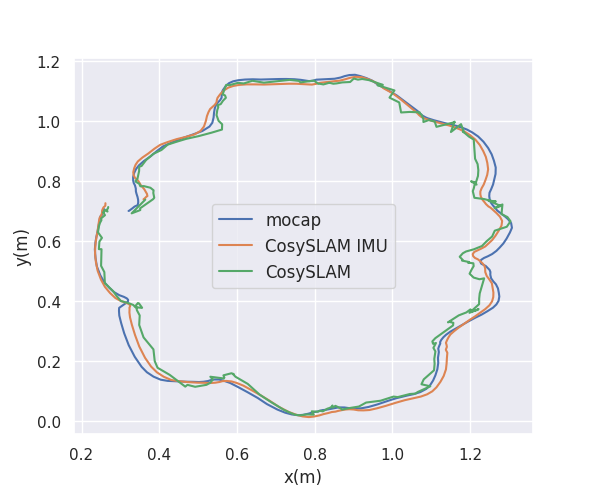
\includegraphics[width=0.9\textwidth]{figures/cosyslam/trajectory_circular.png}
  \caption{Comparison between the MoCap, the output of CosySLAM with visual factors only and the output of CosySLAM with IMU fusion on the circular trajectory.}
  \label{fig:traj_circular}
\end{figure}

In order to validate the performances of the fusion of CosyPose estimates and inertial measurements, we evaluated three scenarios with the camera held by hand and 
T-LESS objects\footnote{T-LESS is one of the datasets for which CosyPose is trained by default and whose object can be bought in the Czech Republic~\cite{hodan17t}. 
It features several small electric devices, whose symmetry at lack of texture make them an interesting benchmark for realistic scenarios.} in the scene. 
The first one is a short and slow trajectory, \ie an ideal scenario. The second one is a slow but long trajectory, to validate the consistency of our system over time. 
The last one is a highly dynamic scenario with a lot of motion that can blur some frames and lose sight of objects for more extended periods. 
Moreover, T-LESS objects being the most difficult objects for pose estimation with CosyPose, they may return many outliers and noisy measurements. 
This is therefore a challenging dataset to test the robustness of our algorithm. \Keyframes\ are selected at 10 Hz, only if objects are detected in the images.

\begin{table}[h]
    \begin{center}
    \caption{Datasets description and results of the hand held videos}
    \label{tab:tless}
    % \begin{tabular}{|c|c{1.1cm}|c{1.1cm}|c{1.1cm}|c{1cm}|}
    \begin{tabular}{|c|c|c|c|c|}
        \hline 
        Scenario  & Length(m) & Duration(s) & MTE¹(cm) & STE²(cm) \\
        \hline 
         V-only - Circular & 3.7 & 23.7 & 3.8 & 1.6\\
        \hline 
         V-only - Short & 2.5 & 12 & 3.8 & 2.4 \\
        \hline 
         V-only - Dynamic & 3.5 & 17.8 & 7.8 & 4.0  \\
        \hline 
         V-IMU - Circular & 3.7 & 23.7 & 1.9 & 0.7\\
        \hline 
         V-IMU - Short & 2.5 & 12 & 1.9 & 0.5 \\
        \hline 
         V-IMU - Dynamic & 3.5 & 17.8 & 1.7 & 1.2  \\
        \hline
    \end{tabular}
    \end{center}
¹ Mean translation error \\
² Standard deviation of translation error
\end{table}

It is interesting to analyze the gains brought by the IMU fusion. The most evident observation is that the output trajectory is smoother, which gives more consistency 
to the result (\figRef{fig:traj_circular}). But we can notice that the MTE is also reduced (\tabRef{tab:tless}). Indeed, the motion model is more precise thanks 
to IMU data. This makes the outlier rejection more efficient than the visual-only CosySLAM which makes a zero velocity assumption between \keyframes.




\subsection{Localization and Mapping of stairs by Solo}

With our retrained model (\secRef{sec:retraining_with_stairs}) we were able to perform SLAM in our experimental area, without augmenting it with other objects. 
We recorded video sequences including stairs with a camera fixed on a Solo robot (\figRef{fig:map_stairs}). A stair has three discrete symmetries 
that are hard to handle for an object pose estimator and the images provided by Solo were noisy because of the walk. 
These scenarios are challenging for our SLAM system, but it maps successfully the stairs and the error on the position of the base of Solo remains reasonable 
(\tabRef{tab:solo}).

\begin{table}[h]
   \begin{center}
   \caption{Datasets description and results of the videos taken on Solo}
   \label{tab:solo}
    % \begin{tabular}{|c{2.2c1cm}|c{1.1cm}|c{1cm}|c{1cm}|}
    \begin{tabular}{|c|c|c|c|c|}
        \hline 
        Scenario  & Length(m) & Duration(s) & MTE(cm) & STE(cm) \\
        \hline 
         V-IMU - Approach & 1.3 & 18.7 & 2.0 & 0.9\\
        \hline 
         V-IMU - Module & 1.3 & 15.5 & 2.4 & 1.5 \\
        \hline
    \end{tabular}
    \end{center}
\end{table}

\begin{figure}[!ht]
  \centering
  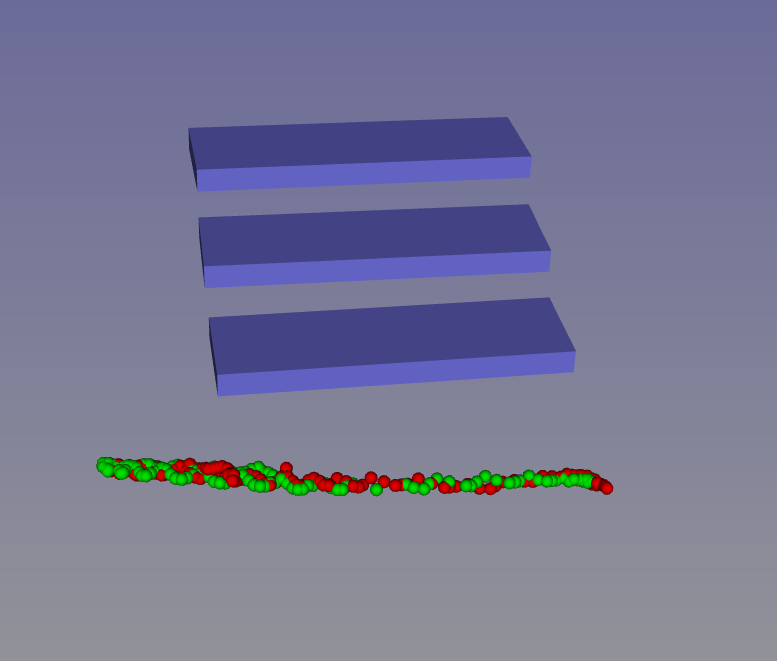
\includegraphics[width=\linewidth]{figures/cosyslam/mapped_stairs.png}
  \caption{This trajectory was recorded on Solo walking along a climbing module made of three stairs using a walking controller \cite{leziart2021implementation}. 
  The green dots represent the trajectory of Solo provided by the MoCap, and the red dots the one produced by our visual-inertial SLAM. 
  The blue rectangles represent the map of the SLAM made of stairs.}
  \label{fig:map_stairs}
\end{figure}




\section{Conclusion}

This chapter presents the first step toward a semantic reconstruction of the robot's environment. We see in this method the potential to provide multi-contact locomotion controllers \cite{carpentier2017multi}
with their needed contact surface reconstructions. By leveraging models of known objects in the scene, one may imagine localizing staircases, their banister, door handles, etc. that
the robot is required to interact with. This work was conducted during the Msc thesis of Cesar Debeunne.

In the case when these object features become sparse, the IMU handles the estimation as a strap-down integration, which is viable for a few seconds. After this delay, extra sources of information are required
to avoid drift in the estimates. One solution would be to increase the robustness of the visual front-end by including residuals using classical 2D salient points features, as visual odometry. In this context,
objects in the scene would be useful both for providing semantic and surface information, as well as providing loop-closures. The covariance model that we developed also requires more development.
In particular, it required important experimental work to build the dataset of CosyPose errors. In particular, needing to collect data for each individual object is very time-consuming. Besides,
the models are likely to overfit the obtained dataset and generalize poorly to datapoints outside of its boundaries.
To improve this, we could work on several aspects. First, the ideal method would be to find a general model, as we did for the AprilTag PnP algorithm (\secRef{sec:apritlag_covariance}), directly computable 
from the CosyPose network. Second, if we show that this is not feasible, we could try to train the covariance model in simulation which provides a vastly superior diversity in situations, though lacking
some of the artifacts of reality. CosyPose itself is only trained in simulation. Thirdly, we could use a Bayesian estimator to fit the uncertainty model, the uncertainty of this model itself in order to 
avoid the particularly bad case of an underestimated covariance. 